% Options for packages loaded elsewhere
\PassOptionsToPackage{unicode}{hyperref}
\PassOptionsToPackage{hyphens}{url}
%
\documentclass[
]{article}
\usepackage{amsmath,amssymb}
\usepackage{setspace}
\usepackage{iftex}
\ifPDFTeX
  \usepackage[T1]{fontenc}
  \usepackage[utf8]{inputenc}
  \usepackage{textcomp} % provide euro and other symbols
\else % if luatex or xetex
  \usepackage{unicode-math} % this also loads fontspec
  \defaultfontfeatures{Scale=MatchLowercase}
  \defaultfontfeatures[\rmfamily]{Ligatures=TeX,Scale=1}
\fi
\usepackage{lmodern}
\ifPDFTeX\else
  % xetex/luatex font selection
\fi
% Use upquote if available, for straight quotes in verbatim environments
\IfFileExists{upquote.sty}{\usepackage{upquote}}{}
\IfFileExists{microtype.sty}{% use microtype if available
  \usepackage[]{microtype}
  \UseMicrotypeSet[protrusion]{basicmath} % disable protrusion for tt fonts
}{}
\usepackage{xcolor}
\usepackage[margin=1in]{geometry}
\usepackage{graphicx}
\makeatletter
\def\maxwidth{\ifdim\Gin@nat@width>\linewidth\linewidth\else\Gin@nat@width\fi}
\def\maxheight{\ifdim\Gin@nat@height>\textheight\textheight\else\Gin@nat@height\fi}
\makeatother
% Scale images if necessary, so that they will not overflow the page
% margins by default, and it is still possible to overwrite the defaults
% using explicit options in \includegraphics[width, height, ...]{}
\setkeys{Gin}{width=\maxwidth,height=\maxheight,keepaspectratio}
% Set default figure placement to htbp
\makeatletter
\def\fps@figure{htbp}
\makeatother
\setlength{\emergencystretch}{3em} % prevent overfull lines
\providecommand{\tightlist}{%
  \setlength{\itemsep}{0pt}\setlength{\parskip}{0pt}}
\setcounter{secnumdepth}{-\maxdimen} % remove section numbering
\newlength{\cslhangindent}
\setlength{\cslhangindent}{1.5em}
\newlength{\csllabelwidth}
\setlength{\csllabelwidth}{3em}
\newlength{\cslentryspacingunit} % times entry-spacing
\setlength{\cslentryspacingunit}{\parskip}
\newenvironment{CSLReferences}[2] % #1 hanging-ident, #2 entry spacing
 {% don't indent paragraphs
  \setlength{\parindent}{0pt}
  % turn on hanging indent if param 1 is 1
  \ifodd #1
  \let\oldpar\par
  \def\par{\hangindent=\cslhangindent\oldpar}
  \fi
  % set entry spacing
  \setlength{\parskip}{#2\cslentryspacingunit}
 }%
 {}
\usepackage{calc}
\newcommand{\CSLBlock}[1]{#1\hfill\break}
\newcommand{\CSLLeftMargin}[1]{\parbox[t]{\csllabelwidth}{#1}}
\newcommand{\CSLRightInline}[1]{\parbox[t]{\linewidth - \csllabelwidth}{#1}\break}
\newcommand{\CSLIndent}[1]{\hspace{\cslhangindent}#1}
\usepackage{lineno}
\usepackage{amsmath}
\numberwithin{equation}
\usepackage{indentfirst}
\linenumbers
\ifLuaTeX
  \usepackage{selnolig}  % disable illegal ligatures
\fi
\IfFileExists{bookmark.sty}{\usepackage{bookmark}}{\usepackage{hyperref}}
\IfFileExists{xurl.sty}{\usepackage{xurl}}{} % add URL line breaks if available
\urlstyle{same}
\hypersetup{
  pdftitle={Environmental warming increases the importance of high-turnover energy channels in stream food webs},
  hidelinks,
  pdfcreator={LaTeX via pandoc}}

\title{Environmental warming increases the importance of high-turnover
energy channels in stream food webs}
\author{true \and true \and true \and true \and true \and true \and true \and true}
\date{}

\begin{document}
\maketitle

\setstretch{1}
Submission journal: Ecology

Submission type: Article

Open Research Statement: All data and code used in this work are
publicly available and archived at Junker (2024) and Zenodo
\url{https://zenodo.org/doi/10.5281/zenodo.10455904}.

Key words: climate change; energy flux; environmental filtering; food
webs; species traits; temperature

\newpage

\hypertarget{abstract}{%
\section{Abstract}\label{abstract}}

Warming temperatures are altering communities and trophic networks
across Earth's ecosystems. While the overall influence of warming on
food webs is often context-dependent, increasing temperatures are
predicted to change communities in two fundamental ways: 1) by reducing
average body size and 2) by increasing individual metabolic rates. These
warming-induced changes have the potential to influence the distribution
of food web fluxes, food web stability, and the relative importance of
deterministic and stochastic ecological processes shaping community
assembly. Here, we quantified patterns and the relative distribution of
organic matter fluxes through stream food webs spanning a broad natural
temperature gradient (5-27\(^\circ\)C). We then related these patterns
to species and community trait distributions of mean body size and
population biomass turnover (\emph{P:B}) within and across streams. We
predicted that 1) communities in warmer streams would exhibit smaller
body size and higher \emph{P:B} and 2) organic matter fluxes within
warmer communities would increasingly skew towards smaller, higher
\emph{P:B} populations. Across the temperature gradient, warmer
communities were characterized by smaller body size (\textasciitilde9\%
per \(^\circ\)C) and higher \emph{P:B} (\textasciitilde7\% faster
turnover per \(^\circ\)C) populations on average. Additionally, organic
matter fluxes \emph{within} warmer streams were increasingly skewed
towards higher \emph{P:B} populations, demonstrating that warming can
restructure organic matter fluxes in both an absolute and relative
sense. With warming, the relative distribution of organic matter fluxes
was decreasingly likely to arise through the random sorting of species,
suggesting stronger selection for traits driving high turnover with
increasing temperature. Our study suggests that a warming world will
favor energy fluxes through `smaller and faster' populations, and that
these changes may be more predictable than previously thought.

\hypertarget{introduction}{%
\section{Introduction}\label{introduction}}

Increasing global temperatures influence the provision and maintenance
of ecosystem services by modifying the network of species interactions
that underpin ecosystem functions (de Ruiter et al. 1995, Woodward et
al. 2010, Brose et al. 2012, Thompson et al. 2012). Warming effects
permeate across multiple levels of biological organization, from control
on individual metabolic rates (Gillooly et al. 2001, Brown et al. 2004)
and biological activity (e.g., attack rate, handling time, growth rates;
Dell et al. 2014), to broad-scale shifts in community assembly and
structure (Nelson et al. 2017b, Gibert 2019, Saito et al. 2021). Across
global climate gradients, such temperature-induced changes have the
potential to mediate food web stability (Baiser et al. 2019) by altering
the acquisition and allocation of resources (Zhang et al. 2017) and the
magnitude and relative distribution of energy fluxes in food webs
(McCann et al. 1998, Gilbert et al. 2014, Barnes et al. 2018).

Understanding how warming alters energy flux in food webs requires
information about how temperature modifies relationships between
ecosystem structure and function. Such relationships depend upon how
warming influences functional trait distributions and how functional
traits translate to the magnitude and distribution of energy demands
(Norberg et al. 2001, Loreau et al. 2001, Norberg 2004). Additionally,
warming can modify community assembly processes (Saito et al.
2021)---both deterministic (e.g., environmental/niche filtering;
Whittaker 1962) and stochastic (e.g., neutral theory; Hubbell
2001)---leading to many possible relationships between warming, the
relative abundance of species, and dominance of particular functional
traits. For example, although temperature appears to have minimal
control on species richness across taxonomic groups (e.g., Bastazini et
al. 2021), warming can have profound effects on the dominance structure
(i.e., evenness) of ecological communities, often by reducing community
evenness and favoring a reduced set of warm-adapted species (Hillebrand
et al. 2008). This strong environmental filtering is likely to skew
trait distributions in natural communities (Therriault and Kolasa 1999).
However, the relative distribution of traits can be further modified by
stochastic processes unrelated to environmental filtering (e.g., species
interactions, Therriault and Kolasa 1999, demographic stochasticity,
Hubbell 2001). The relative importance of these additional processes may
increase with warming, as reduced population abundances (Bernhardt et
al. 2018) and faster metabolic rates increase the possibility of local
extirpation (Siqueira et al. 2020, Saito et al. 2021). The stochastic
shifts in relative species abundances can either exaggerate or counter
any skew in trait distributions driven by environmental filtering and
thereby modify the relationship between species' traits and the absolute
and relative energy demands in food webs.

Body size is a fundamental trait that is influenced by temperature (for
ectotherms see Atkinson 1994, Daufresne et al. 2009, and Gardner et al.
2011, also see Riemer et al. 2018 for deviations across endotherms) and
has great potential to influence energy flux. Reduced body size in
response to warming can arise at multiple levels of organization,
including increased relative abundance of smaller species in warmed
communities (Bergmann 1848), smaller individuals in warmer populations
(James 1970), or reduced absolute body size of warmed individuals
(Atkinson 1994). Thus, warmer communities are likely to contain both
smaller species and individuals. These relationships can have important
implications for energy and material flux in ecosystems because body
size is a strong determinant of species life-history patterns (Peters
1983, Altermatt 2010, Zeuss et al. 2017, Nelson et al. 2020a), as well
as developmental (Angilletta et al. 2004) and metabolic rates (Gillooly
et al. 2001, Brown et al. 2004).

Metabolic rate, in addition to being controlled by body size, is another
key trait that is influenced by temperature and tied to variation in
energy flux through food webs (Gillooly et al. 2001, Barnes et al.
2018). Warming can influence metabolic rates indirectly through
reductions in body size, as well as directly through its effects on
subcellular kinetics (Osmond et al. 2017, Bideault et al. 2019). These
processes can modify ecosystem patterns through changes in population
carrying capacity (Bernhardt et al. 2018) and species relative
abundances, with consequent effects on consumer-resource interactions or
food web structure (Bideault et al. 2019, Gibert 2019). Moreover,
metabolic rates are also tied to many biological processes (Dell et al.
2014), including growth rate (Gillooly et al. 2001), developmental rate
(Zuo et al. 2012, Nelson et al. 2020a), voltinism (Zeuss et al. 2017),
and biomass turnover rate (Brown et al. 2004, Huryn and Benke 2007).
Taken together, these effects suggest that warming should lead to a
smaller, faster world in which ecosystem processes accelerate through
the effects of smaller body size and higher turnover rates, with a
potentially strong imprint on food web structure and energy fluxes
(Gibert 2019).

Here, we address two overarching and open questions focused on
temperature effects on food web dynamics. First, how does ecosystem
temperature shape the relationship between organic matter (OM) fluxes
and community-level trait distributions, specifically body size and
biomass turnover, across ecosystems? Second, how does temperature shape
the role of deterministic vs.~stochastic sorting processes in driving
relative fluxes of OM through consumer communities? We quantified
patterns of OM flux in stream food webs across a natural temperature
gradient (\textasciitilde5--27\(^\circ\)C) in southwestern Iceland.
Previous research in these streams has shown a strong positive effect of
warming on primary production both among streams (Demars et al. 2011,
Padfield et al. 2017) and seasonally within streams (O'Gorman et al.
2012, Hood et al. 2018). Due to high light levels and minimal OM inputs
from surrounding terrestrial habitat, invertebrates in these streams
rely on autochthonous production (O'Gorman et al. 2012, Nelson et al.
2020b); thus, the dynamics of in-stream primary production act as a
strong control on energy flow through consumers (Junker et al. 2020).
Due to the positive relationship of primary production with temperature,
we predicted that annual OM fluxes to consumers would increase with
stream temperature, mirroring patterns in resource availability. We also
hypothesized that temperature would act as a principal environmental
filter on community assembly and OM fluxes by favoring `fast'
life-history traits associated with small-bodied organisms.
Specifically, we predicted that warming temperatures would lead to
reduced average body size and increased average biomass turnover (i.e.,
\emph{Production:Biomass} or \emph{P:B} ratio) of populations among
streams. We also predicted that \emph{within} communities, OM fluxes
would be skewed towards small-bodied and high \emph{P:B} taxa at higher
temperatures, and that these patterns would not arise by random sorting,
but instead through `non-random ordering', suggesting deterministic
filtering of species traits. Our results should help refine general
predictions about how ongoing climate warming, and its influence on key
traits, is likely to shape energy flux through food webs dominated by
ectotherms.

\hypertarget{methods}{%
\section{Methods}\label{methods}}

We studied six streams within the Hengill geothermal field of
southwestern Iceland (64\(^\circ\) 03'N 21\(^\circ\) 18'W) that varied
in mean annual temperature from \textasciitilde5 to 27\(^\circ\)C.
Hengill is characterized by indirect geothermal heating of groundwater
(Árnason et al. 1969), leading to natural variability in stream
temperatures (4.5--54.0 \(^\circ\)C), but similar solute chemistries
(Friberg et al. 2009). These conditions create a ``natural laboratory''
for isolating the effects of temperature on ecosystem processes
(O'Gorman et al. 2014, Nelson et al. 2017b). We selected streams to
maximize the temperature range, while minimizing differences in the
structural aspects of the primary producer community (Junker et al.
2021). However, this did lead to an unequal distribution of streams
along the temperature gradient with three streams concentrated in the
cooler temperature ranges. In each stream, we measured temperature and
water depth every 15 min from July 2010 through August 2012 (U20-001-01
water-level logger, Onset Computer Corp., Pocasset, MA, USA).

\hypertarget{invertebrate-sampling}{%
\subsection{Invertebrate sampling}\label{invertebrate-sampling}}

We sampled macroinvertebrate communities approximately monthly in six
streams, four from July 2011 to August 2012 and two from October 2010 to
October 2011 (\emph{n} = 6 streams). The two streams sampled from
2010--2011 were part of a separate warming manipulation but data for
this study were collected during the un-manipulated reference period
(Nelson et al. 2017a, 2017b). Inter-annual comparisons of primary and
secondary production in previous studies showed minimal differences
among years in un-manipulated streams, suggesting that combining data
from different years would not significantly bias our results (Nelson et
al. 2017a, Hood et al. 2018). We collected five Surber samples (0.023
m\textsuperscript{2}, 250-\(\mu\)m mesh) from randomly selected
locations within each stream encompassing all habitat types. Within the
sampler, inorganic substrates were disturbed to \textasciitilde10 cm
depth and invertebrates and organic matter were removed from stones with
a brush. Samples were then preserved with 5\% formaldehyde until
laboratory analysis. In the laboratory, we split samples into coarse
(\textgreater1 mm) and fine (\textgreater250 \(\mu\)m--\textless1 mm)
fractions using nested sieves and then removed invertebrates from each
fraction under a dissecting microscope (10--15\(\times\) magnification).
For particularly large samples, fine fractions were sub-sampled
(1/2--1/16th) using a modified Folsom plankton splitter prior to removal
of invertebrates. Macroinvertebrates were identified to the lowest
practical taxonomic level (usually genus) with taxonomic keys (Peterson
1977, Merritt et al. 2008, Andersen et al. 2013). Taxon-specific
abundance and biomass were scaled to a per-meter basis by dividing by
the Surber sampler area.

\hypertarget{secondary-production}{%
\subsection{Secondary production}\label{secondary-production}}

Daily secondary production of invertebrate taxa was calculated using the
instantaneous growth rate method (IGR, Benke and Huryn 2017). Growth
rates were determined using taxon-appropriate approaches described in
Junker and others (2020). Briefly, growth rates of common taxa (e.g.,
Chironomidae spp., \emph{Radix balthica}, etc.) were measured using
\emph{in situ} chambers (Huryn and Wallace 1986). Multiple individuals
(\emph{n} = 5--15) within small size categories (\textasciitilde1-mm
length range) were photographed next to a field micrometer, placed in
the stream within pre-conditioned chambers for 7--15 days, and removed
and photographed. Individual lengths were measured from field pictures
using image analysis software (Schindelin et al. 2012), and body lengths
were converted to mass (mg ash-free dry mass {[}AFDM{]}) using published
length-mass regressions (Benke et al. 1999, O'Gorman et al. 2012,
Hannesdóttir et al. 2013). Growth rates (\emph{g},
d\textsuperscript{-1}) were calculated from changes in mean body size
(\emph{M}) over a given time interval (\emph{t}) with the following
equation:

\[g = log_e ( M_{t+\Delta t} / M_t) / \Delta t\] \{\#eq:eqn1\}

Variability in growth rates was estimated by bootstrapping through
repeated resampling of individual lengths with replacement (\emph{n} =
1000). For taxa that exhibit synchronous growth and development (e.g.,
Simuliidae spp., some Chironomidae spp., etc.), we examined temporal
changes in length-frequency distributions and calculated growth rates
and uncertainty using a bootstrap technique similar to that described in
Benke and Huryn (2017). Individual lengths were converted to mass (mg
AFDM) using published length-mass regressions cited above, and
size-frequency histograms were visually inspected for directional
changes in body size through time. For each date, size-frequency
distributions were resampled with replacement and growth rates estimated
from equation 1. We prevented the calculation of negative growth rates
by requiring \(M_{t + \Delta t}\) \textgreater{} \(M_t\). If this
condition was not met after 10,000 resamplings, a minimum growth rate of
0.001 was used (\textless5\% of total instances). To estimate growth
rates of taxa for which growth could not be estimated empirically, we
developed stream-specific growth rate models by constructing
multivariate linear regressions of empirical growth rates against body
size and temperature. To estimate uncertainty in production of each
taxon, we used a bootstrapping technique that resampled measured growth
rates, in addition to abundance and size distributions from individual
samples. For each iteration, size-specific growth rates were multiplied
by mean interval biomass for each size class and the number of days
between sample dates to estimate size class-specific production. For
each time interval, size classes were summed for each taxon to calculate
total population-level interval production. Intervals were summed to
estimate annual secondary production (g AFDM m\textsuperscript{-2}
y\textsuperscript{-1}).

\hypertarget{organic-matter-consumption-estimates}{%
\subsection{Organic matter consumption
estimates}\label{organic-matter-consumption-estimates}}

Organic matter fluxes (g AFDM m\textsuperscript{-2}
y\textsuperscript{-1}) through stream communities were calculated using
the trophic basis of production method (TBP; Benke and Wallace 1980).
Taxon-specific secondary production estimates were combined with diet
proportions, diet-specific assimilation efficiencies,
\emph{AE\textsubscript{i}}, and net production efficiencies, \emph{NPE}
(e.g., McCullough 1975), to estimate consumption of organic matter.
Consumer diets of numerically dominant taxa were quantified through
direct inspection of gut contents from multiple individuals throughout
the year. Removal and preparation of gut tracts followed the methods
outlined in Rosi-Marshall and coauthors (2016). To estimate variability
in diet compositions and to impute missing values for non-dominant taxa,
we modeled the diet proportions within each stream using a hierarchical
multivariate model (Fordyce et al. 2011, Coblentz et al. 2017). Here,
diet proportions for food categories were modeled following a Dirichlet
distribution with expected proportions in diet and a concentration
parameter to estimate variability around this expectation. We accounted
for the hierarchical data structure by fitting stream-specific random
intercepts, as well as random intercept offsets for taxon nested within
each stream. All models were specified in the Stan language (Stan
Development Team 2019) using the \emph{brms} package in R (Bürkner
2017). Further model details can be found in supporting information
(Appendix S1). We estimated diet overlap within and across stream food
webs by calculating diet overlap from 1000 independent draws from the
posterior distributions of modeled diet estimates. Overlap was
calculated with the `overlap()' function in the \emph{RInSp} package
(Zaccarelli et al. 2013).

For each food category, \emph{i}, diet proportions were multiplied by
the gross growth efficiency (\(GGE_{i} = AE_{i} * NPE\)) to calculate
the relative production attributable to each food category. The relative
production from each food type was then multiplied by the interval-level
production and finally divided by \(GGE_{i}\) to estimate consumption of
organic matter from each food category by each taxon (Benke and Wallace
1980). Consumption was calculated for each taxon during each sampling
interval (typically \textasciitilde1 month). Total interval consumption
was calculated by summing across all taxa, while annual consumption was
calculated by summing across all taxa and intervals. Variability in
consumption estimates was estimated through a Monte Carlo approach,
where bootstrapped vectors of secondary production for each taxon (see
\emph{Secondary production} methods above) were resampled and
consumption was estimated with the TBP method using modeled diet
proportions, diet-specific assimilation efficiencies, and net production
efficiency. Variability in \emph{AE\textsubscript{i}} was incorporated
by resampling values from beta distributions fit to median and 2.5\% and
97.5\% percentiles for each diet item: diatoms = 0.30 (95\% percentile
interval {[}PI{]}: 0.24-0.36), filamentous and green algae = 0.30 (95\%
PI: 0.24-0.36), cyanobacteria = 0.10 (95\% PI: 0.08-0.12), amorphous
detritus = 0.10 (95\% PI: 0.08-0.12), vascular and non-vascular plants
(bryophytes) = 0.10 (95\% PI: 0.08-0.12), and animal material = 0.70
(95\% PI: 0.56-0.84; Welch 1968, Benke and Wallace 1980, 1997, Cross et
al. 2007, 2011). Variability in \emph{NPE} was incorporated by
resampling values from an assumed beta distribution with median
\emph{NPE} = 0.45 (95\% PI = 0.40-0.50). Further details can be found in
supporting materials (Appendix S3: Section S1: Trophic basis of
production workflow and assumptions). Beta distributions were fit in R
(R Core Team 2022) using the `get.beta.par()' function within the
\emph{rriskDistributions} package (Belgorodski et al. 2017).

\hypertarget{quantifying-the-distribution-of-food-web-fluxes}{%
\subsection{Quantifying the distribution of food web
fluxes}\label{quantifying-the-distribution-of-food-web-fluxes}}

\hypertarget{evenness-among-taxa}{%
\subsubsection{Evenness among taxa}\label{evenness-among-taxa}}

To visualize and quantify the evenness of OM fluxes, \(p\), among taxa
within each stream, we constructed Lorenz curves (Lorenz 1905) on
rank-ordered OM fluxes, such that in a community with \(S\) species the
relative OM flux of species \emph{j}, \(p_j\), is ordered
\(p_1 \leq p_2 \leq ... p_S\). The Lorenz curve shows how a value, in
this case OM flux, accumulates with an increasing cumulative proportion
of taxa. In a community with an equal distribution of OM flux among
taxa, the Lorenz curve is a straight diagonal line. Deviation from
equality was calculated as the Gini coefficient (Gini 1921), normalized
for differences in \(S\) among streams, \(G^*\) (Solomon 1975, Chao and
Ricotta 2019):

\[ G^* = (2 \sum_{j = 1}^S ip_j -2)/(S-1)\] \{\#eq:eq2\}

where \(G^*\) represents an index of relative evenness of OM fluxes
bounded between zero and one; a value of one represents a community with
equal proportion of total community OM flux for all species (\(1/S\)),
and a value of zero represents a community in which the total OM flux is
attributed to a single taxon.

\hypertarget{distribution-of-om-fluxes-in-relation-to-taxa-traits}{%
\subsubsection{Distribution of OM fluxes in relation to taxa
traits}\label{distribution-of-om-fluxes-in-relation-to-taxa-traits}}

We predicted that warming would favor taxa with smaller body size and
higher biomass turnover rates and that OM fluxes would therefore be
skewed towards small body size (\emph{M}) and higher \emph{P:B} at
higher temperatures across and within communities. To assess the change
in the average population trait values and potential for environmental
filtering across communities, we used bootstrapped linear regressions
between either mean population body size (\(\overline{M}\)) or biomass
turnover (\(\overline{P:B}\)) of each stream community and mean annual
temperature (\(^\circ\)C). Here, 1,000 values of population \emph{M} or
\emph{P:B} were resampled with replacement from population secondary
production vectors (see \emph{Secondary production} above) for each
taxon within each stream. We calculated the mean body size or \emph{P:B}
of the populations within each stream by first calculating the mean
annual body size or annual \emph{P:B} for each taxon and then taking the
median across all taxa. We then calculated the least squares estimate
between log\textsubscript{e}-transformed \(\overline{M}\) or
\(\overline{P:B}\) and mean annual temperature. Response variables were
log\textsubscript{e}-transformed to conform to assumptions of linearity
and normally distributed residual variation and the ordinary least
squares estimate was calculated with the `lm()' function in R.

To quantify how the distribution of organic matter fluxes were modified
\emph{within} communities and whether this modification was related to
temperature, we assessed the extent to which the relative OM fluxes
among taxa were skewed towards populations with lower or higher relative
\emph{M} or \emph{P:B}. To do this, we ordered taxa based on
within-stream rankings of annual population traits (i.e., \emph{M},
\emph{P:B}) and then calculated a measure of skewness, \(Sk_{flux}\),
based on quartiles of the distribution of OM fluxes in relation to taxon
traits as:

\[Sk_{flux} = f_{Q0.75} - 2f_{Q0.5} + f_{Q0.25}/ f_{Q0.75}-f_{Q0.25}\]
\{\#eq:eqn3\}

where \(f_{Qx}\), is the cumulative flux at some quantile, \(Qx\), of
the community trait distribution. We chose this quantile-based formula
over other parametric or moments-based approaches because it is well
defined and requires no assumptions of the moments of the distribution
(Groeneveld and Meeden 1984). We repeated this analysis for all
estimates of OM flux used to calculate \emph{M} and \emph{P:B} in each
stream community. Skewness coefficients range from -1 to 1, where -1
indicates that OM fluxes are skewed perfectly away from a trait while 1
indicates that higher relative fluxes are perfectly associated with
higher trait values. To determine if the skewness of fluxes with
\emph{M} and \emph{P:B} was related to mean annual stream temperature,
we used bootstrapped beta regression with a simple transformation,
\((Sk_{flux} + 1)/2\), to meet the assumptions of the model and
standardize values between 0 and 1. Model coefficients were
back-transformed to estimate effect sizes.

To examine the extent to which temperature influenced the skew of OM
flux among populations within each community, we quantified the
probability of observing the skewed distributions in OM fluxes by random
chance. The feasible range of skewness values within a community is
inherently tied to the evenness of OM fluxes. This dependence on
evenness can make it difficult to determine the importance of random
versus ecological processes on the distribution of OM fluxes by
comparison of raw skewness measures alone. We predicted that species
\(M\) and \(P:B\) would be increasingly important traits structuring OM
fluxes within a community and therefore warmer streams would exhibit
highly skewed OM distributions that would be unlikely due to chance
(i.e., `non-random ordering'). In contrast, cooler streams would exhibit
OM fluxes with skew values that are more likely due to random chance
(`random ordering'), regardless of raw skewness values, suggesting other
traits or processes govern the distribution of OM fluxes within their
communities. To accomplish this, we first had to account for statistical
constraints that restrict the range of possible outcomes (i.e., feasible
set; Haegeman and Loreau 2008, Diaz et al. 2021), given the number of
species and the relative distribution of OM fluxes within a community.
We permuted a random subset of each stream community's feasible set by
randomly ordering species and calculating skewness in the cumulative
distribution of annual OM fluxes 100,000 times in each stream. This
permuted set allowed us to calculate the probability of observing the
empirical skewness value, \(Sk_{flux}\), compared to a random ordering
given the distribution of relative OM flux. We assessed the likelihood
of non-random ordering as the distance from the central mass of the
random skew distributions within each stream. Therefore, communities in
which OM fluxes are likely organized non-randomly are indicated by
observed skew values near the tails of these random distributions.

\hypertarget{results}{%
\section{Results}\label{results}}

\hypertarget{community-organic-matter-fluxes}{%
\subsection{Community organic matter
fluxes}\label{community-organic-matter-fluxes}}

Annual community OM fluxes mirrored patterns of secondary production
reported previously (Junker et al. 2020). Organic matter flux to
invertebrates varied \textasciitilde45-fold among streams, from 3.9 (2.1
-- 6.4; mean {[}95\% Percentile interval{]}) to 176.7 (124.1--236.5) g
AFDM \(m^{-2} y^{-1}\) and was positively related to temperature (Figure
1A).

Differences in OM flux among streams were driven by variation in total
energy demand rather than composition of consumed resources, as consumer
diets were highly similar among streams (Appendix S1: Figure S1). Across
all streams, community-level diets were dominated by diatoms (43.9\%;
c(\texttt{2.5\%} = 0)\%--c(\texttt{97.5\%} = 75.8)\%), amorphous
detritus (17.2\%; c(\texttt{2.5\%} = 0)\%--c(\texttt{97.5\%} = 32.2)\%),
and green algae (13.3\%; c(\texttt{2.5\%} = 0)\%--c(\texttt{97.5\%} =
43)\%). Within streams, diet overlap ranged from 68\% (65\%--71\%) to
75\% (69\%--79\%) among invertebrate taxa. Among streams, diets were
also highly similar with a mean overlap of 89\% (85\%--92\%). Diet
overlap based on pairwise comparisons among streams showed little
difference and no clear relationship with temperature.

\hypertarget{evenness-of-organic-matter-fluxes}{%
\subsection{Evenness of organic matter
fluxes}\label{evenness-of-organic-matter-fluxes}}

In general, OM fluxes were unevenly distributed among taxa (Gini
inequality coefficients ranged from 0.09 {[}0.07 -- 0.11, 95\% PI{]} to
0.29 {[}0.25 -- 0.32{]}; Appendix S2: Table S1) and were dominated by
insects in the families Simuliidae and Chironomidae, pulmonate snails
(\emph{Radix balthica}), and oligochaete worms (Figure 2A \& B; Appendix
S2: Figure S2). In absolute terms, \textasciitilde85\% of total OM flux
was contributed by 2 to 10 taxa, which comprised only 3\% to 29\% of
total taxon richness among streams. Although differences in evenness
among streams were partially attributed to variation in taxon richness
(range: 14 to 35), fluxes were still highly uneven after accounting for
differences in richness (i.e., similar `Normalized' Gini coefficients,
Appendix S2: Table S1). As average stream temperature increased, OM
fluxes shifted from dominance by Simuliidae in the coolest stream to
Chironomidae and \emph{R. balthica} at moderate temperatures (Figure
2A). In the warmest stream, where maximum temperatures can often
approach \textasciitilde40\(^\circ\)C, taxon richness was lowest and OM
fluxes were dominated by oligochaete worms in the family Naididae, the
chironomid \emph{Cricotopus sylvestris}, and \emph{R. balthica} (Figure
2A). Among-stream differences in evenness of OM fluxes were not clearly
related to temperature (Appendix S2: Table S1).

\hypertarget{organic-matter-fluxes-in-relation-to-body-size-and-biomass-turnover-rate}{%
\subsection{Organic matter fluxes in relation to body size and biomass
turnover
rate}\label{organic-matter-fluxes-in-relation-to-body-size-and-biomass-turnover-rate}}

Across stream communities, average population body size
(\(\overline{M}\); mg AFDM ind\textsuperscript{-1}) decreased and
average population biomass turnover rate (\(\overline{P:B}\);
y\textsuperscript{-1}) increased with increasing temperature (Figure 1B
\& C). \(\overline{M}\) decreased from 2.75 mg AFDM
ind\textsuperscript{-1} (c(\texttt{2.5\%} = 1.03) -- c(\texttt{97.5\%} =
5.08); 95\% PI) in the coldest stream to 0.10 mg AFDM
ind\textsuperscript{-1} (c(\texttt{2.5\%} = 0.08) -- c(\texttt{97.5\%} =
0.13)) in the warmest stream, corresponding to an -8.7\% (-11.1 -- -6.4)
change in mean body size for every 1\(^\circ\)C increase in temperature
(Figure 1B). \(\overline{P:B}\) ratio increased from 4.4
y\textsuperscript{-1} (c(\texttt{2.5\%} = 3.6) -- c(\texttt{97.5\%} =
5.1)) in the coldest stream to 35.5 y\textsuperscript{-1}
(c(\texttt{2.5\%} = 29.6) -- c(\texttt{97.5\%} = 43.3)) in the warmest
stream corresponding to a 6.9\% (6.1--7.9) increase in
\(\overline{P:B}\) ratio for every 1\(^\circ\)C increase (Figure 1C).

Within stream communities, there were diverse body size--OM flux
relationships, with some streams showing greater relative OM flux
through larger-bodied taxa (positive skew), others showing greater OM
flux through smaller-bodied taxa (negative skew), and some that showed
no size-related trend in OM flux (skew range: c(\texttt{50\%} = -1) to
c(\texttt{50\%} = 0.56); Figure 3A \& B). Skew estimates of OM fluxes in
relation to body size showed little association with stream temperature
except in the warmest stream, where fluxes were heavily skewed toward
small-bodied taxa (Figure 3B). Similarly, skew in OM fluxes in relation
to \emph{P:B} ratios varied among streams, ranging from c(\texttt{50\%}
= -0.4) to c(\texttt{50\%} = 1). In this case, OM fluxes to consumers
skewed increasingly toward higher turnover (\emph{P:B}) taxa with
increasing temperature (Figure 4A \& B).

We compared our skew estimates (i.e., \(Sk_{flux}\)) of OM flux based on
ordered data (i.e., ordered from small to large \emph{M} or low to high
\emph{P:B} ratios; Figure 3B and Figure 4B) to skew estimates based on
randomly sorted data to detect whether OM fluxes through smaller and
higher \emph{P:B} taxa could be attributed to these traits instead of
random community assembly processes. The probability of observing a
similar or more extreme skew of OM fluxes in relation to body size was
variable among streams and ranged from 0.34 (c(\texttt{2.5\%} =
0.19)--c(\texttt{97.5\%} = 0.55); 95\% PI) to 0.79 (c(\texttt{2.5\%} =
0.07)--c(\texttt{97.5\%} = 0.96)); there was little association between
this probability and temperature (Figure 3C). In contrast, the
probability of a similar or more extreme skew in relation to \emph{P:B}
ratios ranged from 0.06 (c(\texttt{2.5\%} = 0)--c(\texttt{97.5\%} =
0.75)) to 0.62 (c(\texttt{2.5\%} = 0.23)--c(\texttt{97.5\%} = 0.81);
Figure 4C) and in this case there was a clear trend towards a more
structured OM flux distribution---i.e., fluxes through high \emph{P:B}
taxa were favored at higher temperatures. The likelihood of higher
relative fluxes among high \emph{P:B} taxa became much higher with
warming, and the probability of random ordering decreased by -4.6\%
(-5.1\%---4.2\%) for every 1\(^\circ\)C increase in temperature (Figure
4C).

\hypertarget{discussion}{%
\section{Discussion}\label{discussion}}

While a growing body of theoretical and empirical research has enhanced
our knowledge of temperature-mediated changes to ecosystems (e.g.,
O'Connor et al. 2009), general patterns remain elusive and empirical
studies often show idiosyncratic outcomes (Nelson et al. 2017a, Zhang et
al. 2017), especially at higher levels of biological organization
(Walther et al. 2002, Woodward et al. 2010). Here, we demonstrate that
warming acts as a strong environmental filter of species traits along a
wide natural gradient of ecosystem temperatures. In particular, we found
that increasing temperatures were associated with reduced population
body size and increased population biomass turnover among stream
invertebrate communities, leading to higher organic matter fluxes
through these populations. In addition, we found that higher
temperatures systematically skewed OM fluxes \emph{within} communities,
such that OM flows were increasingly dominated by taxa with rapid
life-cycles. Lastly, we discovered that the distribution of fluxes
within communities was non-random, especially with respect to \emph{P:B}
ratios at moderate to high temperatures, suggesting that temperature was
especially important in structuring relative performance and resource
acquisition within warm communities. These patterns show that the
acceleration of energy and material fluxes through ecosystems in both an
absolute (among ecosystems) and relative (within ecosystems) sense may
be a general effect of environmental warming.

\hypertarget{across-stream-trends-in-community-overlinepb-and-overlinem}{%
\subsection{\texorpdfstring{Across-stream trends in community
\(\overline{P:B}\) and
\(\overline{M}\)}{Across-stream trends in community \textbackslash overline\{P:B\} and \textbackslash overline\{M\}}}\label{across-stream-trends-in-community-overlinepb-and-overlinem}}

Warming-induced shifts in community body size distributions were
associated with a community-level increase in the absolute rates of
material flux. At the community level, we observed a \textasciitilde7\%
increase in the mean biomass turnover rate (\emph{P:B};
y\textsuperscript{-1}) of populations for each 1\(^\circ\)C of warming.
Although this effect among communities may be partially attributed to
the thermodynamic influence of temperature (Gillooly et al. 2001),
biomass turnover rate is also closely related to organism body size
(Brown et al. 2004, Huryn and Benke 2007). Thus, warming may influence
the distributions of \emph{P:B} ratios directly through its effects on
metabolic rate and indirectly through reductions in organism body size
and associated life-history traits. The increase in \emph{P:B} we
observed across communities was similar in magnitude to the reduction in
body size (i.e., +7\% vs --9\%, respectively), reinforcing the
fundamental connection between organism body size and \emph{P:B}, but
also suggesting increases in mean population \emph{P:B} across
communities may, in part, be attributed to reduced organism body sizes
(Figure 1B \& C). Organism body size is related to a number of other
ecological attributes (Peters 1983) and changes in body size with
increasing temperatures are likely to have broad implications for
ecosystems in a changing climate (Gibert 2019).

A general reduction in body size has been deemed a ``universal''
response to warming (Daufresne et al. 2009, Gardner et al. 2011, Uszko
et al. 2022), but notable deviations exist across ecosystems (Thresher
et al. 2007, O'Gorman et al. 2012, Ohlberger 2013). Based on our monthly
sampling over a full annual cycle, we observed a clear decrease in the
average body size of populations from cool to warm communities (Figure
1B), corresponding to a \textasciitilde9\% decline in the mass of
individuals for every 1\(^\circ\)C increase in temperature. While this
change is based on community-level shifts (i.e., different sets of
taxa), the magnitude of decline is consistent with intra-taxon patterns
measured across broad phylogenetic groups (Deutsch et al. 2022).
Interestingly, our results contrast with a warming experiment conducted
in one of our study streams showing that a relatively small increase in
temperature (3\(^\circ\)C) shifted invertebrate community biomass and
productivity from smaller to larger organisms (Nelson et al. 2017a,
2017b). Moreover, an additional study at Hengill that examined community
size spectra across a much broader range of body sizes and taxonomic
groups (i.e., diatoms to fish), but with limited temporal sampling
(i.e., August only), reported an unexpected shallowing of mass-abundance
slopes, suggesting warming may favor larger-bodied individuals (Adams et
al. 2013, O'Gorman et al. 2017). Other studies have reported similar
deviations from the ``universal'' response for other taxonomic groups
(e.g., invertebrates: Zeuss et al. 2017, birds: Geist 1987, Riemer et
al. 2018, fish: Rypel 2014). While there is a strong propensity for
reduced body size with warming, clearly many processes can modify the
direction and magnitude of body size shifts and how they play out from
individual to ecosystem levels (e.g., growth and developmental rates,
resource supply, competition, predation; Ohlberger 2013). In addition,
it is evident that the range of temperatures and body sizes considered,
as well as the temporal scale of sampling, is likely to influence our
understanding of how temperature influences patterns of body size in
ecosystems (Jennings et al. 2007).

\hypertarget{relative-om-fluxes-in-relation-to-species-trait-distributions}{%
\subsection{Relative OM fluxes in relation to species trait
distributions}\label{relative-om-fluxes-in-relation-to-species-trait-distributions}}

In addition to the cross-ecosystem effects of temperature on patterns of
species traits and organic matter flux, we found that temperature had
strong effects on the relative performance of species \emph{within}
communities, leading to an increase in OM fluxes through populations
with high biomass turnover rates. Generally speaking, OM fluxes were
unevenly distributed among populations within communities, which may be
expected given the systematic unevenness in the distribution of
individuals among species (Diaz et al. 2021). However, we found
important residual structure in the unevenness of OM fluxes that
appeared to be related to functional trait axes. With respect to body
size, the results were somewhat equivocal. In the coldest and warmest
streams, we saw a strong skew in material fluxes towards larger and
smaller species, respectively, but this pattern was not apparent at
moderate temperatures (\textasciitilde6--17\(^\circ\)C). In contrast, we
found a much clearer pattern with respect to biomass turnover rates, in
which OM fluxes were increasingly skewed towards taxa with high turnover
within warmer streams. We also found that this pattern was clearly
non-random, suggesting that it is not likely to have arisen from
stochastic, neutral processes alone (e.g., Hubbell 2001, Shoemaker et
al. 2020). These results suggest that temperature may be a strong
environmental filter---and therefore natural selection agent---for taxa
with high turnover rates and associated life-history traits (e.g.,
multi-voltinism: Zeuss et al. 2017, Nelson et al. 2020a, short lifespan:
Munch and Salinas 2009, Stoks et al. 2014, high growth rate: Donhauser
et al. 2020), especially at relatively high temperatures.

\hypertarget{warming-and-resource-interactions}{%
\subsection{Warming and resource
interactions}\label{warming-and-resource-interactions}}

The ecological and evolutionary effects of warming are likely mediated
by their interaction with food resource availability and dynamics (Cross
et al. 2015, McMeans et al. 2015). In high-latitude ecosystems where
light plays a dominant role in driving resource dynamics, consumer
energy demands may be affected by resources more than by temperature
\emph{per se} (Huryn and Benstead 2019, Junker et al. 2020). This may be
particularly apparent in open-canopied streams where primary production
is highly synchronous with seasonal light regimes. Under such
conditions, simplified resource dynamics may create strong selection for
high growth and turnover rates (and associated \emph{r}-selected
life-history traits, such as small body size) because consumers cannot
compensate for periods of resource scarcity through diet shifts (e.g.,
consumptive ``portfolio'' effects, Gutgesell et al. 2022). Future
warming may exaggerate these effects because ectotherms may experience
increased temperature-driven energy demands that are increasingly
decoupled from resource availability (Huryn and Benstead 2019).
Acknowledging these dynamics may lead to a more general framework for
understanding different responses to warming across organisms
(Greyson-Gaito et al. 2023), latitudes (Gibert 2019), and ecosystem
types (McMeans et al. 2015, Gutgesell et al. 2022).

\hypertarget{conclusions}{%
\subsection{Conclusions}\label{conclusions}}

We documented the important role of temperature in structuring key
functional traits and the relative distribution of material fluxes
across a natural stream temperature gradient. Higher temperatures were
associated with increased total flux through the food web, as well as
reductions in average population body size and increases in population
biomass turnover. Further, biomass turnover rate---but less so body
size---was increasingly important for structuring OM fluxes at warmer
temperatures. Our results support the idea that warming may reduce
organism size and also `speed up' ecosystem dynamics in both an absolute
and relative sense. These changes have important implications for the
maintenance of biodiversity, as well as for the connections between
biodiversity and the magnitude and stability of ecosystem energy and
material cycles in a warming world.

\hypertarget{acknowledgements}{%
\section{Acknowledgements}\label{acknowledgements}}

We are grateful to Sigurður Guðjónsson, Guðni Guðbergsson, and the staff
at the Veiðimálastofnun for providing laboratory space and logistical
support. We are also grateful to Sveinbjörn Steinþorsson at the
University of Iceland for super-jeep transport to our field sites during
the winter. We thank Lauren David, David Hernandez, Amanda Keasberry,
Elena Nava, Camille Perrett, Jackie Pitts, Friðþjófur Árnason, Liliana
García, Ragnahildur Magnúsdottír, Ryan McClure, Vija Pelekis, Adam
Toomey, Chau Tran, Brooke Weigel, Tanner Williamson and many
undergraduate workers for field and laboratory help. Jeff Wesner and Abe
Kanz generously provided R code and discussions on modeling diet
proportions. We thank Dr.~Victor Saito and one anonymous reviewer for
constructive comments that improved the paper. This study was supported
by the National Science Foundation (DEB-0949774 and DEB-1354624 to JPB
and ADH and DEB-0949726 to WFC).

\hypertarget{conflict-of-interest}{%
\section{Conflict of Interest}\label{conflict-of-interest}}

The authors have no conflict of interest to declare.

\hypertarget{references}{%
\section{References}\label{references}}

\hypertarget{refs}{}
\begin{CSLReferences}{1}{0}
\leavevmode\vadjust pre{\hypertarget{ref-adams2013}{}}%
Adams, G. L., D. E. Pichler, E. J. Cox, E. J. O'Gorman, A. Seeney, G.
Woodward, and D. C. Reuman. 2013.
\href{https://doi.org/10.1111/gcb.12285}{Diatoms can be an important
exception to temperature--size rules at species and community levels of
organization}. Global Change Biology 19:3540--3552.

\leavevmode\vadjust pre{\hypertarget{ref-altermatt2010}{}}%
Altermatt, F. 2010.
\href{https://doi.org/10.1098/rspb.2009.1910}{Climatic warming increases
voltinism in {European} butterflies and moths}. Proceedings of the Royal
Society B: Biological Sciences 277:1281--1287.

\leavevmode\vadjust pre{\hypertarget{ref-andersen2013}{}}%
Andersen, T., P. S. Cranston, and J. H. Epler. 2013. Chironomidae of the
{Holarctic} region: {Keys} and diagnoses, {Part} 1. Media Tryck, Lund,
Sweden.

\leavevmode\vadjust pre{\hypertarget{ref-angilletta2004}{}}%
Angilletta, M. J., Jr., T. D. Steury, and M. W. Sears. 2004.
\href{https://doi.org/10.1093/icb/44.6.498}{Temperature, {Growth Rate},
and {Body Size} in {Ectotherms}: {Fitting Pieces} of a {Life-History
Puzzle}}. Integrative and Comparative Biology 44:498--509.

\leavevmode\vadjust pre{\hypertarget{ref-arnason1969}{}}%
Árnason, B., P. Theodorsson, S. Björnsson, and K. Saemundsson. 1969.
\href{https://doi.org/10.1007/BF02596720}{Hengill, a high temperature
thermal area in {Iceland}}. Bulletin Volcanologique 33:245--259.

\leavevmode\vadjust pre{\hypertarget{ref-atkinson1994}{}}%
Atkinson, D. 1994. Temperature and organism size: A biological law for
ectotherms? Advances in ecological research 25:1--58.

\leavevmode\vadjust pre{\hypertarget{ref-baiser2019}{}}%
Baiser, B., D. Gravel, A. R. Cirtwill, J. A. Dunne, A. K. Fahimipour, L.
J. Gilarranz, J. A. Grochow, D. Li, N. D. Martinez, A. McGrew, T.
Poisot, T. N. Romanuk, D. B. Stouffer, L. B. Trotta, F. S. Valdovinos,
R. J. Williams, S. A. Wood, and J. D. Yeakel. 2019.
\href{https://doi.org/10.1111/geb.12925}{Ecogeographical rules and the
macroecology of food webs}. Global Ecology and Biogeography
28:1204--1218.

\leavevmode\vadjust pre{\hypertarget{ref-barnes2018}{}}%
Barnes, A. D., M. Jochum, J. S. Lefcheck, N. Eisenhauer, C. Scherber, M.
I. O'Connor, P. de Ruiter, and U. Brose. 2018.
\href{https://doi.org/10.1016/j.tree.2017.12.007}{Energy {Flux}: {The
Link} between {Multitrophic Biodiversity} and {Ecosystem Functioning}}.
Trends in Ecology \& Evolution 33:186--197.

\leavevmode\vadjust pre{\hypertarget{ref-bastazini2021}{}}%
Bastazini, V. A. G., N. Galiana, H. Hillebrand, M. Estiarte, R. Ogaya,
J. Peñuelas, U. Sommer, and J. M. Montoya. 2021.
\href{https://doi.org/10.1111/geb.13308}{The impact of climate warming
on species diversity across scales: {Lessons} from experimental
meta-ecosystems}. Global Ecology and Biogeography 30:1545--1554.

\leavevmode\vadjust pre{\hypertarget{ref-belgorodski2017}{}}%
Belgorodski, N., M. Greiner, K. Tolksdorf, and K. Schueller. 2017.
{rriskDistributions}: {Fitting Distributions} to {Given Data} or {Known
Quantiles}.

\leavevmode\vadjust pre{\hypertarget{ref-benke2017}{}}%
Benke, A. C., and A. D. Huryn. 2017. Secondary production and
quantitative food webs. Pages 235--254 Methods in {Stream Ecology}.
Elsevier.

\leavevmode\vadjust pre{\hypertarget{ref-benke1999}{}}%
Benke, A. C., A. D. Huryn, L. A. Smock, and J. B. Wallace. 1999.
\href{https://doi.org/10.2307/1468447}{Length-{Mass Relationships} for
{Freshwater Macroinvertebrates} in {North America} with {Particular
Reference} to the {Southeastern United States}}. Journal of the North
American Benthological Society 18:308--343.

\leavevmode\vadjust pre{\hypertarget{ref-benke1980}{}}%
Benke, A. C., and J. B. Wallace. 1980.
\href{https://doi.org/10.2307/1937161}{Trophic {Basis} of {Production
Among Net-Spinning Caddisflies} in a {Southern Appalachian Stream}}.
Ecology 61:108--118.

\leavevmode\vadjust pre{\hypertarget{ref-benke1997}{}}%
Benke, A. C., and J. B. Wallace. 1997.
\href{https://doi.org/10.1890/0012-9658(1997)078\%5B1132:TBOPAR\%5D2.0.CO;2}{Trophic
{Basis} of {Production Among Riverine Caddisflies}: {Implications} for
{Food Web Analysis}}. Ecology 78:1132--1145.

\leavevmode\vadjust pre{\hypertarget{ref-bergmann1848}{}}%
Bergmann, C. 1848. {Ü}ber die {Verh{ä}ltnisse} der {W{ä}rme{ö}konomie}
der {Thiere} zu ihrer {Gr{ö}sse}.

\leavevmode\vadjust pre{\hypertarget{ref-bernhardt2018}{}}%
Bernhardt, J. R., J. M. Sunday, and M. I. O'Connor. 2018.
\href{https://doi.org/10.1086/700114}{Metabolic {Theory} and the
{Temperature-Size Rule Explain} the {Temperature Dependence} of
{Population Carrying Capacity}}. The American Naturalist:000--000.

\leavevmode\vadjust pre{\hypertarget{ref-bideault2019}{}}%
Bideault, A., M. Loreau, and D. Gravel. 2019.
\href{https://doi.org/10.3389/fevo.2019.00045}{Temperature {Modifies
Consumer-Resource Interaction Strength Through Its Effects} on
{Biological Rates} and {Body Mass}}. Frontiers in Ecology and Evolution
7.

\leavevmode\vadjust pre{\hypertarget{ref-brose2012}{}}%
Brose, U., J. A. Dunne, Montoya José M., O. L. Petchey, F. D. Schneider,
and U. Jacob. 2012.
\href{https://doi.org/10.1098/rstb.2012.0232}{Climate change in
size-structured ecosystems}. Philosophical Transactions of the Royal
Society B: Biological Sciences 367:2903--2912.

\leavevmode\vadjust pre{\hypertarget{ref-brown2004}{}}%
Brown, J. H., J. F. Gillooly, A. P. Allen, V. M. Savage, and G. B. West.
2004. \href{https://doi.org/10.1890/03-9000}{Toward a {Metabolic Theory}
of {Ecology}}. Ecology 85:1771--1789.

\leavevmode\vadjust pre{\hypertarget{ref-burkner2017}{}}%
Bürkner, P.-C. 2017. \href{https://doi.org/10.18637/jss.v080.i01}{Brms:
{An R Package} for {Bayesian Multilevel Models Using Stan}}. Journal of
Statistical Software 80:1--28.

\leavevmode\vadjust pre{\hypertarget{ref-chao2019}{}}%
Chao, A., and C. Ricotta. 2019.
\href{https://doi.org/10.1002/ecy.2852}{Quantifying evenness and linking
it to diversity, beta diversity, and similarity}. Ecology 100:e02852.

\leavevmode\vadjust pre{\hypertarget{ref-coblentz2017}{}}%
Coblentz, K. E., A. E. Rosenblatt, and M. Novak. 2017.
\href{https://doi.org/10.1002/ecy.1802}{The application of {Bayesian}
hierarchical models to quantify individual diet specialization}. Ecology
98:1535--1547.

\leavevmode\vadjust pre{\hypertarget{ref-cross2011}{}}%
Cross, W. F., C. V. Baxter, K. C. Donner, E. J. Rosi-Marshall, T. A.
Kennedy, R. O. Hall, H. A. W. Kelly, and R. S. Rogers. 2011.
\href{https://doi.org/10.1890/10-1719.1}{Ecosystem ecology meets
adaptive management: Food web response to a controlled flood on the
{Colorado River}, {Glen Canyon}}. Ecological Applications 21:2016--2033.

\leavevmode\vadjust pre{\hypertarget{ref-cross2015}{}}%
Cross, W. F., J. M. Hood, J. P. Benstead, A. D. Huryn, and D. Nelson.
2015. \href{https://doi.org/10.1111/gcb.12809}{Interactions between
temperature and nutrients across levels of ecological organization}.
Global Change Biology 21:1025--1040.

\leavevmode\vadjust pre{\hypertarget{ref-cross2007}{}}%
Cross, W. F., J. B. Wallace, and A. D. Rosemond. 2007.
\href{https://doi.org/10.1890/06-1348.1}{Nutrient {Enrichment Reduces
Constraints} on {Material Flows} in a {Detritus-Based Food Web}}.
Ecology 88:2563--2575.

\leavevmode\vadjust pre{\hypertarget{ref-daufresne2009}{}}%
Daufresne, M., K. Lengfellner, and U. Sommer. 2009.
\href{https://doi.org/10.1073/pnas.0902080106}{Global warming benefits
the small in aquatic ecosystems}. Proceedings of the National Academy of
Sciences 106:12788--12793.

\leavevmode\vadjust pre{\hypertarget{ref-deruiter1995}{}}%
de Ruiter, P. C., A.-M. Neutel, and J. C. Moore. 1995.
\href{https://doi.org/10.1126/science.269.5228.1257}{Energetics,
{Patterns} of {Interaction Strengths}, and {Stability} in {Real
Ecosystems}}. Science 269:1257--1260.

\leavevmode\vadjust pre{\hypertarget{ref-dell2014}{}}%
Dell, A. I., S. Pawar, and V. M. Savage. 2014.
\href{https://doi.org/10.1111/1365-2656.12081}{Temperature dependence of
trophic interactions are driven by asymmetry of species responses and
foraging strategy}. Journal of Animal Ecology 83:70--84.

\leavevmode\vadjust pre{\hypertarget{ref-demars2011}{}}%
Demars, B. O. L., J. R. Manson, J. S. Ólafsson, G. M. Gíslason, R.
Gudmundsdóttir, G. Woodward, J. Reiss, D. E. Pichler, J. J. Rasmussen,
and N. Friberg. 2011.
\href{https://doi.org/10.1111/j.1365-2427.2010.02554.x}{Temperature and
the metabolic balance of streams}. Freshwater Biology 56:1106--1121.

\leavevmode\vadjust pre{\hypertarget{ref-deutsch2022}{}}%
Deutsch, C., J. L. Penn, W. C. E. P. Verberk, K. Inomura, M.-G. Endress,
and J. L. Payne. 2022.
\href{https://doi.org/10.1073/pnas.2201345119}{Impact of warming on
aquatic body sizes explained by metabolic scaling from microbes to
macrofauna}. Proceedings of the National Academy of Sciences
119:e2201345119.

\leavevmode\vadjust pre{\hypertarget{ref-diaz2021a}{}}%
Diaz, R. M., H. Ye, and S. K. M. Ernest. 2021.
\href{https://doi.org/10.1111/ele.13820}{Empirical abundance
distributions are more uneven than expected given their statistical
baseline}. Ecology Letters n/a.

\leavevmode\vadjust pre{\hypertarget{ref-donhauser2020}{}}%
Donhauser, J., P. A. Niklaus, J. Rousk, C. Larose, and B. Frey. 2020.
\href{https://doi.org/10.1016/j.soilbio.2020.107873}{Temperatures beyond
the community optimum promote the dominance of heat-adapted, fast
growing and stress resistant bacteria in alpine soils}. Soil Biology and
Biochemistry 148:107873.

\leavevmode\vadjust pre{\hypertarget{ref-fordyce2011}{}}%
Fordyce, J. A., Z. Gompert, M. L. Forister, and C. C. Nice. 2011.
\href{https://doi.org/10.1371/journal.pone.0026785}{A {Hierarchical
Bayesian Approach} to {Ecological Count Data}: {A Flexible Tool} for
{Ecologists}}. PLOS ONE 6:e26785.

\leavevmode\vadjust pre{\hypertarget{ref-friberg2009}{}}%
Friberg, N., J. B. Dybkjær, J. S. Olafsson, G. M. Gislason, S. E.
Larsen, and T. L. Lauridsen. 2009.
\href{https://doi.org/10.1111/j.1365-2427.2009.02234.x}{Relationships
between structure and function in streams contrasting in temperature}.
Freshwater Biology 54:2051--2068.

\leavevmode\vadjust pre{\hypertarget{ref-gardner2011}{}}%
Gardner, J. L., A. Peters, M. R. Kearney, L. Joseph, and R. Heinsohn.
2011. \href{https://doi.org/10.1016/j.tree.2011.03.005}{Declining body
size: A third universal response to warming?} Trends in Ecology \&
Evolution 26:285--291.

\leavevmode\vadjust pre{\hypertarget{ref-geist1987}{}}%
Geist, V. 1987. \href{https://doi.org/10.1139/z87-164}{Bergmann's rule
is invalid}. Canadian Journal of Zoology.

\leavevmode\vadjust pre{\hypertarget{ref-gibert2019}{}}%
Gibert, J. P. 2019.
\href{https://doi.org/10.1038/s41598-019-41783-0}{Temperature directly
and indirectly influences food web structure}. Scientific Reports
9:5312.

\leavevmode\vadjust pre{\hypertarget{ref-gilbert2014}{}}%
Gilbert, B., T. D. Tunney, K. S. McCann, J. P. DeLong, D. A. Vasseur, V.
Savage, J. B. Shurin, A. I. Dell, B. T. Barton, C. D. G. Harley, H. M.
Kharouba, P. Kratina, J. L. Blanchard, C. Clements, M. Winder, H. S.
Greig, and M. I. O'Connor. 2014.
\href{https://doi.org/10.1111/ele.12307}{A bioenergetic framework for
the temperature dependence of trophic interactions}. Ecology Letters
17:902--914.

\leavevmode\vadjust pre{\hypertarget{ref-gillooly2001}{}}%
Gillooly, J. F., J. H. Brown, G. B. West, V. M. Savage, and E. L.
Charnov. 2001. \href{https://doi.org/10.1126/science.1061967}{Effects of
size and temperature on metabolic rate}. Science (New York, N.Y.)
293:2248--2251.

\leavevmode\vadjust pre{\hypertarget{ref-gini1921}{}}%
Gini, C. 1921. \href{https://doi.org/10.2307/2223319}{Measurement of
{Inequality} of {Incomes}}. The Economic Journal 31:124--126.

\leavevmode\vadjust pre{\hypertarget{ref-greyson-gaito2023}{}}%
Greyson-Gaito, C. J., G. Gellner, and K. S. McCann. 2023.
\href{https://doi.org/10.1098/rspb.2022.2149}{Life-history speed,
population disappearances and noise-induced ratchet effects}.
Proceedings of the Royal Society B: Biological Sciences 290:20222149.

\leavevmode\vadjust pre{\hypertarget{ref-groeneveld1984}{}}%
Groeneveld, R. A., and G. Meeden. 1984.
\href{https://doi.org/10.2307/2987742}{Measuring {Skewness} and
{Kurtosis}}. The Statistician 33:391.

\leavevmode\vadjust pre{\hypertarget{ref-gutgesell2022a}{}}%
Gutgesell, M. K., K. S. McCann, G. Gellner, K. Cazelles, C. J.
Greyson-Gaito, C. Bieg, M. M. Guzzo, C. P. K. Warne, C. A. Ward, R. F.
O'Connor, A. M. Scott, B. C. Graham, E. J. Champagne, and B. C. McMeans.
2022. \href{https://doi.org/10.1093/biosci/biab144}{On the {Dynamic
Nature} of {Omnivory} in a {Changing World}}. BioScience 72:416--430.

\leavevmode\vadjust pre{\hypertarget{ref-haegeman2008}{}}%
Haegeman, B., and M. Loreau. 2008.
\href{https://doi.org/10.1111/j.1600-0706.2008.16539.x}{Limitations of
entropy maximization in ecology}. Oikos 117:1700--1710.

\leavevmode\vadjust pre{\hypertarget{ref-hannesdottir2013}{}}%
Hannesdóttir, E. R., G. M. Gíslason, J. S. Ólafsson, Ó. P. Ólafsson, and
E. J. O'Gorman. 2013.
\href{https://doi.org/10.1016/B978-0-12-417199-2.00005-7}{Increased
{Stream Productivity} with {Warming Supports Higher Trophic Levels}}.
Advances in Ecological Research 48:285--342.

\leavevmode\vadjust pre{\hypertarget{ref-hillebrand2008}{}}%
Hillebrand, H., D. M. Bennett, and M. W. Cadotte. 2008.
\href{https://doi.org/10.1890/07-1053.1}{Consequences of dominance: A
review of evenness effects on local and regional ecosystem processes}.
Ecology 89:1510--1520.

\leavevmode\vadjust pre{\hypertarget{ref-hood2018}{}}%
Hood, J. M., J. P. Benstead, W. F. Cross, A. D. Huryn, P. W. Johnson, G.
M. Gíslason, J. R. Junker, D. Nelson, J. S. Ólafsson, and C. Tran. 2018.
\href{https://doi.org/10.1111/gcb.13912}{Increased resource use
efficiency amplifies positive response of aquatic primary production to
experimental warming}. Global Change Biology 24:1069--1084.

\leavevmode\vadjust pre{\hypertarget{ref-hubbell2001}{}}%
Hubbell, S. P. 2001. The unified neutral theory of biodiversity and
biogeography. Princeton University Press.

\leavevmode\vadjust pre{\hypertarget{ref-huryn2007}{}}%
Huryn, A. D., and A. C. Benke. 2007. Relationship between biomass
turnover and body size for stream communities. Body size: the structure
and function of aquatic ecosystems. Cambridge University Press,
Cambridge, UK:55--76.

\leavevmode\vadjust pre{\hypertarget{ref-huryn2019}{}}%
Huryn, A. D., and J. P. Benstead. 2019.
\href{https://doi.org/10.1002/ecy.2690}{Seasonal changes in light
availability modify the temperature dependence of secondary production
in an {Arctic} stream}. Ecology 100:e02690.

\leavevmode\vadjust pre{\hypertarget{ref-huryn1986}{}}%
Huryn, A. D., and J. B. Wallace. 1986.
\href{https://doi.org/10.4319/lo.1986.31.1.0216}{A method for obtaining
in situ growth rates of larval {Chironomidae} ({Diptera}) and its
application to studies of secondary production}. Limnology and
Oceanography 31:216--221.

\leavevmode\vadjust pre{\hypertarget{ref-james1970}{}}%
James, F. C. 1970. \href{https://doi.org/10.2307/1935374}{Geographic
{Size Variation} in {Birds} and {Its Relationship} to {Climate}}.
Ecology 51:365--390.

\leavevmode\vadjust pre{\hypertarget{ref-jennings2007}{}}%
Jennings, S., J. a. a. D. Oliveira, and K. J. Warr. 2007.
\href{https://doi.org/10.1111/j.1365-2656.2006.01180.x}{Measurement of
body size and abundance in tests of macroecological and food web
theory}. Journal of Animal Ecology 76:72--82.

\leavevmode\vadjust pre{\hypertarget{ref-junkerEnergyFlux}{}}%
Junker, J. 2024, January.
\href{https://doi.org/10.5281/zenodo.10455905}{Jimjunker1/{Junker}\_temperature-energy-flux}.
Zenodo.

\leavevmode\vadjust pre{\hypertarget{ref-junker2020}{}}%
Junker, J. R., W. F. Cross, J. P. Benstead, A. D. Huryn, J. M. Hood, D.
Nelson, G. M. Gíslason, and J. S. Ólafsson. 2020.
\href{https://doi.org/10.1111/ele.13608}{Resource supply governs the
apparent temperature dependence of animal production in stream
ecosystems}. Ecology Letters 23:1809--1819.

\leavevmode\vadjust pre{\hypertarget{ref-junker2021}{}}%
Junker, J. R., W. F. Cross, J. P. Benstead, A. D. Huryn, J. M. Hood, D.
Nelson, G. M. Gíslason, and J. S. Ólafsson. 2021.
\href{https://doi.org/10.1007/s10021-020-00585-6}{Flow is more
{Important} than {Temperature} in {Driving Patterns} of {Organic Matter
Storage} and {Stoichiometry} in {Stream Ecosystems}}. Ecosystems
24:1317--1331.

\leavevmode\vadjust pre{\hypertarget{ref-loreau2001}{}}%
Loreau, M., S. Naeem, P. Inchausti, J. Bengtsson, J. P. Grime, A.
Hector, D. U. Hooper, M. A. Huston, D. Raffaelli, B. Schmid, D. Tilman,
and D. A. Wardle. 2001.
\href{https://doi.org/10.1126/science.1064088}{Biodiversity and
{Ecosystem Functioning}: {Current Knowledge} and {Future Challenges}}.
Science 294:804--808.

\leavevmode\vadjust pre{\hypertarget{ref-lorenz1905}{}}%
Lorenz, M. O. 1905. \href{https://doi.org/10.2307/2276207}{Methods of
{Measuring} the {Concentration} of {Wealth}}. Publications of the
American Statistical Association 9:209.

\leavevmode\vadjust pre{\hypertarget{ref-mccann1998}{}}%
McCann, K., A. Hastings, and G. R. Huxel. 1998.
\href{https://doi.org/10.1038/27427}{Weak trophic interactions and the
balance of nature}. Nature 395:794--798.

\leavevmode\vadjust pre{\hypertarget{ref-mccullough1975}{}}%
McCullough, D. A. 1975.
\href{https://doi.org/10.2172/7299553}{Bioenergetics of three aquatic
insects determined by radioisotopic analyses}.

\leavevmode\vadjust pre{\hypertarget{ref-mcmeans2015}{}}%
McMeans, B. C., K. S. McCann, M. Humphries, N. Rooney, and A. T. Fisk.
2015. \href{https://doi.org/10.1016/j.tree.2015.09.001}{Food {Web
Structure} in {Temporally-Forced Ecosystems}}. Trends in Ecology \&
Evolution 30:662--672.

\leavevmode\vadjust pre{\hypertarget{ref-merritt2008}{}}%
Merritt, R. W., K. W. Cummins, and M. B. Berg, editors. 2008. An
{Introduction} to the {Aquatic Insects} of {North America}. 4th edition.
Kendall/Hunt Publishing Co., Dubuque, IA.

\leavevmode\vadjust pre{\hypertarget{ref-munch2009}{}}%
Munch, S. B., and S. Salinas. 2009.
\href{https://doi.org/10.1073/pnas.0900300106}{Latitudinal variation in
lifespan within species is explained by the metabolic theory of
ecology}. Proceedings of the National Academy of Sciences
106:13860--13864.

\leavevmode\vadjust pre{\hypertarget{ref-nelson2017}{}}%
Nelson, D., J. P. Benstead, A. D. Huryn, W. F. Cross, J. M. Hood, P. W.
Johnson, J. R. Junker, G. M. Gíslason, and J. S. Ólafsson. 2017a.
\href{https://doi.org/10.1002/ecy.1857}{Shifts in community size
structure drive temperature invariance of secondary production in a
stream-warming experiment}. Ecology 98:1797--1806.

\leavevmode\vadjust pre{\hypertarget{ref-nelson2017a}{}}%
Nelson, D., J. P. Benstead, A. D. Huryn, W. F. Cross, J. M. Hood, P. W.
Johnson, J. R. Junker, G. M. Gíslason, and J. S. Ólafsson. 2017b.
\href{https://doi.org/10.1111/gcb.13574}{Experimental whole-stream
warming alters community size structure}. Global Change Biology
23:2618--2628.

\leavevmode\vadjust pre{\hypertarget{ref-nelson2020}{}}%
Nelson, D., J. P. Benstead, A. D. Huryn, W. F. Cross, J. M. Hood, P. W.
Johnson, J. R. Junker, G. M. Gíslason, and J. S. Ólafsson. 2020b.
\href{https://doi.org/10.1002/ecy.2952}{Thermal niche diversity and
trophic redundancy drive neutral effects of warming on energy flux
through a stream food web}. Ecology.

\leavevmode\vadjust pre{\hypertarget{ref-nelson2020b}{}}%
Nelson, D., J. P. Benstead, A. D. Huryn, W. F. Cross, J. M. Hood, P. W.
Johnson, J. R. Junker, G. M. Gíslason, and J. S. Ólafsson. 2020a.
\href{https://doi.org/10.1111/fwb.13583}{Contrasting responses of black
fly species ({Diptera}: {Simuliidae}) to experimental whole-stream
warming}. Freshwater Biology 65:1793--1805.

\leavevmode\vadjust pre{\hypertarget{ref-norberg2004}{}}%
Norberg, J. 2004.
\href{https://doi.org/10.4319/lo.2004.49.4_part_2.1269}{Biodiversity and
ecosystem functioning: {A} complex adaptive systems approach}. Limnology
and Oceanography 49:1269--1277.

\leavevmode\vadjust pre{\hypertarget{ref-norberg2001}{}}%
Norberg, J., D. P. Swaney, J. Dushoff, J. Lin, R. Casagrandi, and S. A.
Levin. 2001. \href{https://doi.org/10.1073/pnas.171315998}{Phenotypic
diversity and ecosystem functioning in changing environments: {A}
theoretical framework}. Proceedings of the National Academy of Sciences
98:11376--11381.

\leavevmode\vadjust pre{\hypertarget{ref-oconnor2009}{}}%
O'Connor, M. I., M. F. Piehler, D. M. Leech, A. Anton, and J. F. Bruno.
2009. \href{https://doi.org/10.1371/journal.pbio.1000178}{Warming and
{Resource Availability Shift Food Web Structure} and {Metabolism}}. PLOS
Biology 7:e1000178.

\leavevmode\vadjust pre{\hypertarget{ref-ogorman2014}{}}%
O'Gorman, E. J., J. P. Benstead, W. F. Cross, N. Friberg, J. M. Hood, P.
W. Johnson, B. D. Sigurdsson, and G. Woodward. 2014.
\href{https://doi.org/10.1111/gcb.12602}{Climate change and geothermal
ecosystems: Natural laboratories, sentinel systems, and future refugia}.
Global Change Biology 20:3291--3299.

\leavevmode\vadjust pre{\hypertarget{ref-ogorman2012}{}}%
O'Gorman, E. J., D. E. Pichler, G. Adams, J. P. Benstead, H. Cohen, N.
Craig, W. F. Cross, B. O. L. Demars, N. Friberg, G. M. Gíslason, R.
Gudmundsdóttir, A. Hawczak, J. M. Hood, L. N. Hudson, L. Johansson, M.
P. Johansson, J. R. Junker, A. Laurila, J. R. Manson, E. Mavromati, D.
Nelson, J. S. Ólafsson, D. M. Perkins, O. L. Petchey, M. Plebani, D. C.
Reuman, B. C. Rall, R. Stewart, M. S. A. Thompson, and G. Woodward.
2012. \href{https://doi.org/10.1016/B978-0-12-398315-2.00002-8}{Impacts
of {Warming} on the {Structure} and {Functioning} of {Aquatic
Communities}}. Pages 81--176 Advances in {Ecological Research}.
Elsevier.

\leavevmode\vadjust pre{\hypertarget{ref-ogorman2017}{}}%
O'Gorman, E. J., L. Zhao, D. E. Pichler, G. Adams, N. Friberg, B. C.
Rall, A. Seeney, H. Zhang, D. C. Reuman, and G. Woodward. 2017.
\href{https://doi.org/10.1038/nclimate3368}{Unexpected changes in
community size structure in a natural warming experiment}. Nature
Climate Change 7:659--663.

\leavevmode\vadjust pre{\hypertarget{ref-ohlberger2013}{}}%
Ohlberger, J. 2013.
\href{https://doi.org/10.1111/1365-2435.12098}{Climate warming and
ectotherm body size -- from individual physiology to community ecology}.
Functional Ecology 27:991--1001.

\leavevmode\vadjust pre{\hypertarget{ref-osmond2017}{}}%
Osmond, M. M., M. A. Barbour, J. R. Bernhardt, M. W. Pennell, J. M.
Sunday, and M. I. O'Connor. 2017.
\href{https://doi.org/10.1086/691387}{Warming-{Induced Changes} to {Body
Size Stabilize Consumer-Resource Dynamics}}. The American Naturalist
189:718--725.

\leavevmode\vadjust pre{\hypertarget{ref-padfield2017}{}}%
Padfield, D., C. Lowe, A. Buckling, R. Ffrench-Constant, S. Jennings, F.
Shelley, J. S. Ólafsson, and G. Yvon-Durocher. 2017.
\href{https://doi.org/10.1111/ele.12820}{Metabolic compensation
constrains the temperature dependence of gross primary production}.
Ecology Letters 20:1250--1260.

\leavevmode\vadjust pre{\hypertarget{ref-peters1983}{}}%
Peters, R. H. 1983. \href{https://doi.org/10.1017/CBO9780511608551}{The
ecological implications of body size}. Cambridge University Press,
Cambridge.

\leavevmode\vadjust pre{\hypertarget{ref-peterson1977}{}}%
Peterson, B. V. 1977. Black flies of {Iceland} ({Diptera-Simuliidae}).
Canadian Entomologist 109:449--472.

\leavevmode\vadjust pre{\hypertarget{ref-rcoreteam2022}{}}%
R Core Team. 2022. R: {A Language} and {Environment} for {Statistical
Computing}. R Foundation for Statistical Computing, Vienna, Austria.

\leavevmode\vadjust pre{\hypertarget{ref-riemer2018}{}}%
Riemer, K., R. P. Guralnick, and E. P. White. 2018.
\href{https://doi.org/10.7554/eLife.27166}{No general relationship
between mass and temperature in endothermic species}. eLife 7:e27166.

\leavevmode\vadjust pre{\hypertarget{ref-rosi-marshall2016}{}}%
Rosi-Marshall, E. J., H. A. Wellard Kelly, R. O. Hall, and K. A. Vallis.
2016. \href{https://doi.org/10.1086/684648}{Methods for quantifying
aquatic macroinvertebrate diets}. Freshwater Science 35:229--236.

\leavevmode\vadjust pre{\hypertarget{ref-rypel2014}{}}%
Rypel, A. L. 2014. \href{https://doi.org/10.1086/674094}{The {Cold-Water
Connection}: {Bergmann}'s {Rule} in {North American Freshwater Fishes}}.
The American Naturalist 183:147--156.

\leavevmode\vadjust pre{\hypertarget{ref-saito2021}{}}%
Saito, V. S., D. M. Perkins, and P. Kratina. 2021.
\href{https://doi.org/10.1016/j.tree.2021.01.003}{A {Metabolic
Perspective} of {Stochastic Community Assembly}}. Trends in Ecology \&
Evolution:S0169534721000057.

\leavevmode\vadjust pre{\hypertarget{ref-schindelin2012}{}}%
Schindelin, J., I. Arganda-Carreras, E. Frise, V. Kaynig, M. Longair, T.
Pietzsch, S. Preibisch, C. Rueden, S. Saalfeld, B. Schmid, J.-Y.
Tinevez, D. J. White, V. Hartenstein, K. Eliceiri, P. Tomancak, and A.
Cardona. 2012. \href{https://doi.org/10.1038/nmeth.2019}{Fiji: An
open-source platform for biological-image analysis}. Nature Methods
9:676--682.

\leavevmode\vadjust pre{\hypertarget{ref-shoemaker2020}{}}%
Shoemaker, L. G., L. L. Sullivan, I. Donohue, J. S. Cabral, R. J.
Williams, M. M. Mayfield, J. M. Chase, C. Chu, W. S. Harpole, A. Huth,
J. HilleRisLambers, A. R. M. James, N. J. B. Kraft, F. May, R.
Muthukrishnan, S. Satterlee, F. Taubert, X. Wang, T. Wiegand, Q. Yang,
and K. C. Abbott. 2020.
\href{https://doi.org/10.1002/ecy.2922}{Integrating the underlying
structure of stochasticity into community ecology}. Ecology 101:e02922.

\leavevmode\vadjust pre{\hypertarget{ref-siqueira2020}{}}%
Siqueira, T., V. S. Saito, L. M. Bini, A. S. Melo, D. K. Petsch, V. L.
Landeiro, K. T. Tolonen, J. Jyrkänkallio-Mikkola, J. Soininen, and J.
Heino. 2020. \href{https://doi.org/10.1002/ecy.3014}{Community size can
affect the signals of ecological drift and niche selection on
biodiversity}. Ecology 101.

\leavevmode\vadjust pre{\hypertarget{ref-solomon1975}{}}%
Solomon, D. L. 1975. A comparative approach to species diversity. Page
7. Technical \{\{Report\}\}, Biometrics Unit, Cornell University,
Ithaca, NY USA.

\leavevmode\vadjust pre{\hypertarget{ref-stan2019}{}}%
Stan Development Team. 2019. Stan {Modeling Language Users Guide} and
{Reference Manual}.

\leavevmode\vadjust pre{\hypertarget{ref-stoks2014}{}}%
Stoks, R., A. N. Geerts, and L. De Meester. 2014.
\href{https://doi.org/10.1111/eva.12108}{Evolutionary and plastic
responses of freshwater invertebrates to climate change: Realized
patterns and future potential}. Evolutionary Applications 7:42--55.

\leavevmode\vadjust pre{\hypertarget{ref-therriault1999}{}}%
Therriault, T. W., and J. Kolasa. 1999. Physical determinants of
richness, diversity, evenness and abundance in natural aquatic
microcosms. Oecologia 412:123--130.

\leavevmode\vadjust pre{\hypertarget{ref-thompson2012}{}}%
Thompson, R. M., U. Brose, J. A. Dunne, R. O. Hall, S. Hladyz, R. L.
Kitching, N. D. Martinez, H. Rantala, T. N. Romanuk, D. B. Stouffer, and
J. M. Tylianakis. 2012.
\href{https://doi.org/10.1016/j.tree.2012.08.005}{Food webs: Reconciling
the structure and function of biodiversity}. Trends in Ecology \&
Evolution 27:689--697.

\leavevmode\vadjust pre{\hypertarget{ref-thresher2007}{}}%
Thresher, R. E., J. A. Koslow, A. K. Morison, and D. C. Smith. 2007.
\href{https://doi.org/10.1073/pnas.0610546104}{Depth-mediated reversal
of the effects of climate change on long-term growth rates of exploited
marine fish}. Proceedings of the National Academy of Sciences
104:7461--7465.

\leavevmode\vadjust pre{\hypertarget{ref-uszko2022}{}}%
Uszko, W., M. Huss, and A. Gårdmark. 2022.
\href{https://doi.org/10.1002/ecy.3699}{Smaller species but larger
stages: {Warming} effects on inter- and intraspecific community size
structure}. Ecology 103:e3699.

\leavevmode\vadjust pre{\hypertarget{ref-walther2002}{}}%
Walther, G.-R., E. Post, P. Convey, A. Menzel, C. Parmesan, T. J. C.
Beebee, J.-M. Fromentin, O. Hoegh-Guldberg, and F. Bairlein. 2002.
\href{https://doi.org/10.1038/416389a}{Ecological responses to recent
climate change}. Nature 416:389--395.

\leavevmode\vadjust pre{\hypertarget{ref-welch1968}{}}%
Welch, H. E. 1968. \href{https://doi.org/10.2307/1935541}{Relationships
between {Assimiliation Efficiencies} and {Growth Efficiencies} for
{Aquatic Consumers}}. Ecology 49:755--759.

\leavevmode\vadjust pre{\hypertarget{ref-whittaker1962}{}}%
Whittaker, R. H. 1962.
\href{https://doi.org/10.1007/BF02860872}{Classification of natural
communities}. The Botanical Review 28:1--239.

\leavevmode\vadjust pre{\hypertarget{ref-woodward2010}{}}%
Woodward, G., J. P. Benstead, O. S. Beveridge, J. Blanchard, T. Brey, L.
E. Brown, W. F. Cross, N. Friberg, T. C. Ings, U. Jacob, S. Jennings, M.
E. Ledger, A. M. Milner, J. M. Montoya, E. O'Gorman, J. M. Olesen, O. L.
Petchey, D. E. Pichler, D. C. Reuman, M. S. A. Thompson, F. J. F. Van
Veen, and G. Yvon-Durocher. 2010.
\href{https://doi.org/10.1016/B978-0-12-381363-3.00002-2}{Ecological
{Networks} in a {Changing Climate}}. Pages 71--138 Advances in
{Ecological Research}. Elsevier.

\leavevmode\vadjust pre{\hypertarget{ref-zaccarelli2013}{}}%
Zaccarelli, N., D. I. Bolnick, and G. Mancinelli. 2013.
\href{https://doi.org/10.1111/2041-210X.12079}{{RInSp}: An r package for
the analysis of individual specialization in resource use}. Methods in
Ecology and Evolution 4:1018--1023.

\leavevmode\vadjust pre{\hypertarget{ref-zeuss2017}{}}%
Zeuss, D., S. Brunzel, and R. Brandl. 2017.
\href{https://doi.org/10.1111/geb.12525}{Environmental drivers of
voltinism and body size in insect assemblages across {Europe}}. Global
Ecology and Biogeography 26:154--165.

\leavevmode\vadjust pre{\hypertarget{ref-zhang2017}{}}%
Zhang, L., D. Takahashi, M. Hartvig, and K. H. Andersen. 2017.
\href{https://doi.org/10.1098/rspb.2017.1772}{Food-web dynamics under
climate change}. Proceedings of the Royal Society B: Biological Sciences
284:20171772.

\leavevmode\vadjust pre{\hypertarget{ref-zuo2012}{}}%
Zuo, W., M. E. Moses, G. B. West, C. Hou, and J. H. Brown. 2012.
\href{https://doi.org/10.1098/rspb.2011.2000}{A general model for
effects of temperature on ectotherm ontogenetic growth and development}.
Proceedings of the Royal Society B: Biological Sciences 279:1840--1846.

\end{CSLReferences}

\newpage

\hypertarget{figure-captions}{%
\section{Figure captions}\label{figure-captions}}

Figure 1. (a) Total organic matter flux (g AFDM m\textsuperscript{-2}
y\textsuperscript{-1}) increased with mean annual temperature. Higher
stream temperatures also led to (b) a decrease in mean population body
size (\(\overline{M}\), mg ind\textsuperscript{-1}) and (c) an increase
in mean population biomass turnover rate (\(\overline{P:B}\),
y\textsuperscript{-1}). For all panels, points represent the mean value,
wide bars represent the 25\textsuperscript{th} and
75\textsuperscript{th} percentile bounds, narrow bars represent the
2.5\textsuperscript{th} and 97.5\textsuperscript{th} percentile bounds,
and grey lines show a random sample of bootstrapped linear models (n =
400).

Figure 2. (a) Percent contribution of taxa to OM flux
(log\textsubscript{e}{[}g AFDM m\textsuperscript{-2}
y\textsuperscript{-1}{]})in each stream; colors correspond to mean
annual temperature shown in the legend; (b) rank-ordered organic matter
flux (log\textsubscript{e}{[}g AFDM m\textsuperscript{-2}
y\textsuperscript{-1}{]}) by taxon. Taxon abbreviations: F:Naid, Family
Naididae; N comm, \emph{Nais communis}; C syl, \emph{Cricotopus
sylvestris}; R balt, \emph{Radix balthica}; Macro sp.,
\emph{Macropelopia} sp.; C dent, \emph{Chaetocladius dentiforceps}; S
vitt, \emph{Simulium vittatum}; Euk spp., \emph{Eukiefferiella} spp.; O
obl, \emph{Orthocladius oblidens}; Micro sp. \emph{Micropsectra} sp.; D
bert, \emph{Diamesa bertrami}; D boh-zer, \emph{Diamesa
bohemani-zernyi}; F: Lumb, Family Lumbricidae; P cing,
\emph{Potamophylax cingulatus}; S gland, \emph{Sperchon glandulosus}; P
urs, \emph{Prosimulium ursinum}; SC: Cope, Subclass Copepoda; R eff,
\emph{Rheocricotopus effusus}; S vern, \emph{Simulium vernum}; Chaet
sp., \emph{Chaetocladius} sp.; Thien sp., \emph{Thienemanniella} sp.; O
frig, \emph{Orthocladius frigidus}; Limn rip, \emph{Limnophora riparia};
Dicra, \emph{Dicranota} sp.; C: Ost, Class Ostracoda; S aur,
\emph{Simulium aureum}. The number of taxa represented in the ``Other''
category for each stream is shown in the lower right corner of each
panel.

Figure 3. (a) Lorenz curves showing cumulative relative organic matter
flux among taxa with increasing body size (from left to right; \emph{M},
mg AFDM ind\textsuperscript{-1}). The solid line 1:1 line from the
origin represents the line of equality. Distributions near this line
suggest minimal structuring of OM fluxes in relation to body size. The
dotted line allows for visualization of skewness in OM fluxes based on
its intersection with the empirical Lorenz curve. (b) Empirical
estimates of body size-related OM flux skewness in relation to stream
temperature. (c) The probability of observing these skewness values when
compared to a random ordering. For panels B and C, points represent the
median value, wide bars represent the 25\textsuperscript{th} and
75\textsuperscript{th} percentile bounds, and narrow bars represent the
2.5\textsuperscript{th} and 97.5\textsuperscript{th} percentile bounds.

Figure 4. (a) Lorenz curves showing cumulative relative organic matter
flux among taxa with increasing \emph{P:B} ratio (from left to right;
y\textsuperscript{-1}). The solid 1:1 line from the origin represents
the line of equality. Distributions near this line suggest minimal
structuring of OM fluxes in relation to \emph{P:B} ratio. The dotted
line allows for visualization of skewness in OM fluxes based on its
intersection with the Lorenz curve. (b) Estimates of \emph{P:B}-related
OM flux skewness in relation to stream temperature. (c) The probability
of observing these skewness values when compared to a random (i.e.,
stochastic) ordering. For panels B and C, points represent the median
value, wide bars represent the 25\textsuperscript{th} and
75\textsuperscript{th} percentile bounds, and narrow bars represent the
2.5\textsuperscript{th} and 97.5\textsuperscript{th} percentile bounds.

\newpage

Figure 1

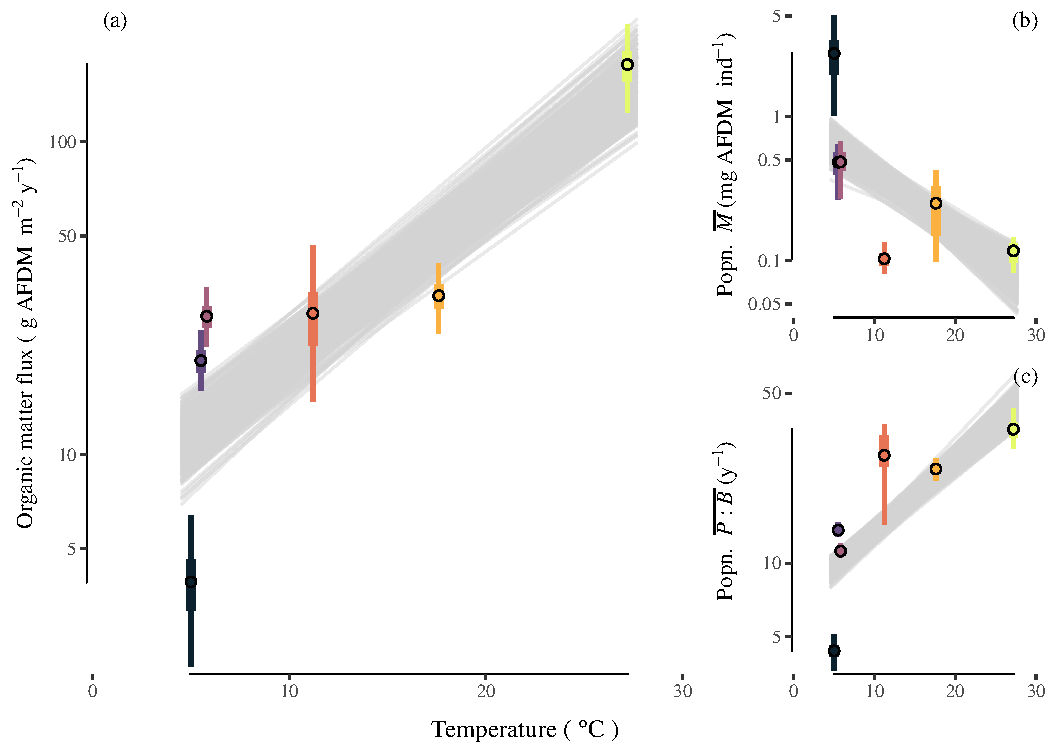
\includegraphics{Junker_temp-energy-flux_accepted_files/figure-latex/figure 1-1.pdf}

\newpage

Figure 2

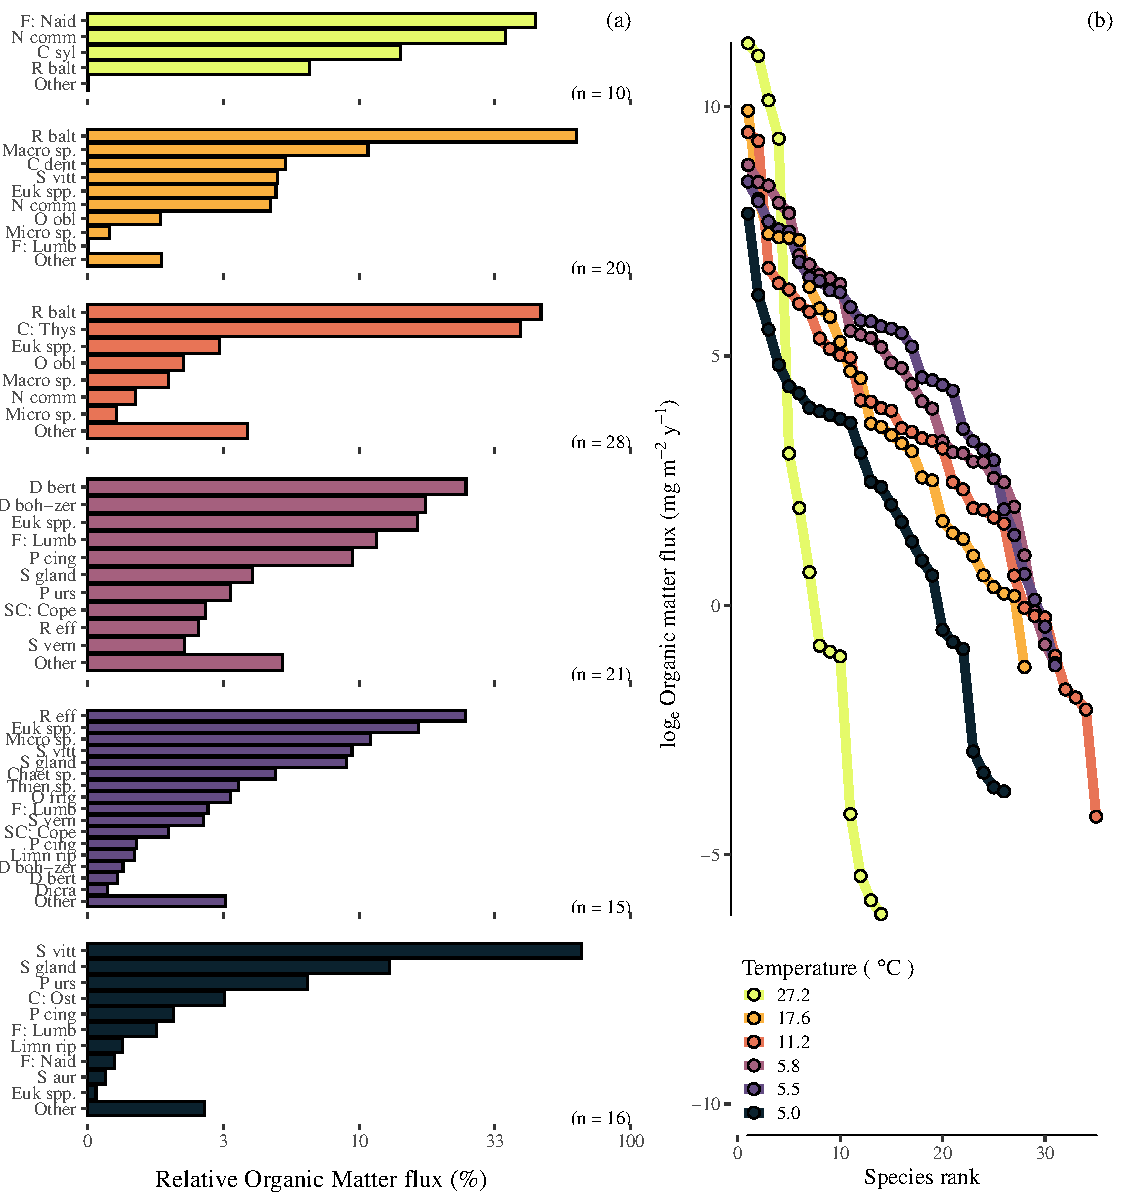
\includegraphics{Junker_temp-energy-flux_accepted_files/figure-latex/figure 2-1.pdf}

\newpage

Figure 3

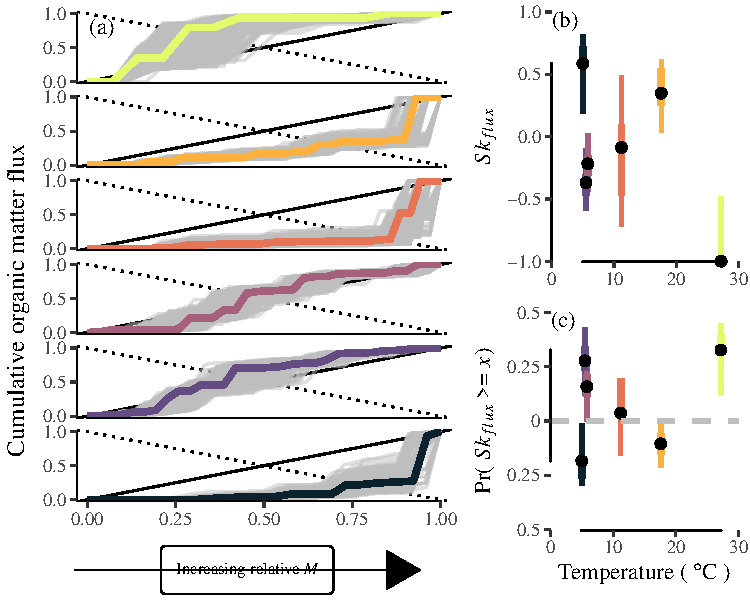
\includegraphics{Junker_temp-energy-flux_accepted_files/figure-latex/figure 3-1.pdf}

\newpage

Figure 4

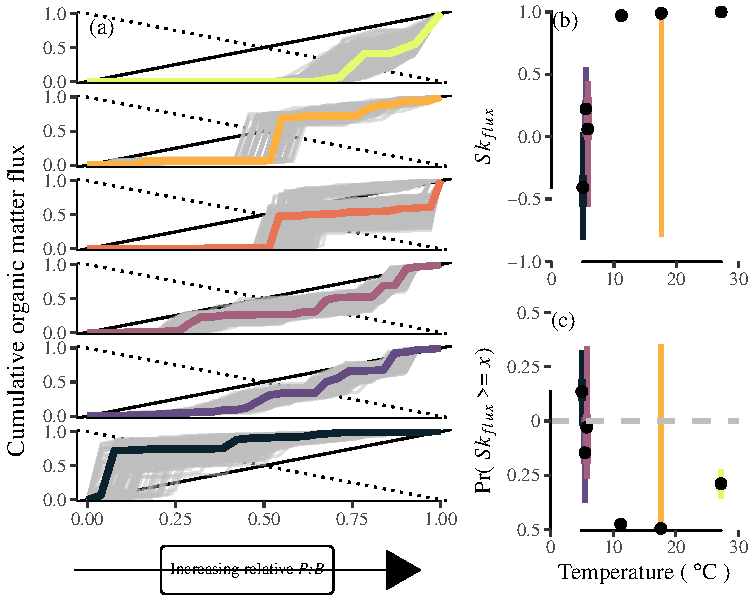
\includegraphics{Junker_temp-energy-flux_accepted_files/figure-latex/figure 4-1.pdf}

\end{document}
